
%% ECSE 420 -- Project proposal

%
\documentclass[conference]{IEEEtran}
%
% If IEEEtran.cls has not been installed into the LaTeX system files,
% manually specify the path to it like:
% \documentclass[conference]{../sty/IEEEtran}


%My packages
\usepackage{graphicx}
\graphicspath{{./figures/}}
\usepackage[xetex,colorlinks=true,urlcolor = black, 
linkcolor=black,citecolor=black]{hyperref}


% correct bad hyphenation here
\hyphenation{op-tical net-works semi-conduc-tor}


\begin{document}
% paper title
% can use linebreaks \\ within to get better formatting as desired
\title{ECSE 548 - Project Proposal:\\8-bit Booth Multiplier}

%\vspace{-20pt}
\author{\IEEEauthorblockN{Marco Kassis,
Aryan Mojtahedi,
Dimitrios Stamoulis and
Louis-Charles Trudeau}
\IEEEauthorblockA{Department of Electrical and Computer Engineering\\
McGill University, Montreal, Canada}}


% make the title area
\maketitle
\IEEEpeerreviewmaketitle

%~\\
%\vspace{+10pt}
\section{Introduction}
\IEEEPARstart{T}{he} current document is the 
submitted Project Proposal for the 
ECSE 548: Introduction to VLSI Systems	
course. Our project team (\texttt{myCourses-Group 4}) 
consists of Mr Marco Kassis, Mr Aryan Mojtahedi, Mr Dimitrios Stamoulis and
Mr Louis-Charles Trudeau. A brief description of 
the intended project follows. 
%\hfill October 09, 2013



\section{Intended result of the project}
\subsection{System to be designed}

The selected system to be
designed is the 8-bit Booth Multiplier \cite{booth}\cite{macS}. 
Standard static logic CMOS will be used. 
The principles of the \emph{Booth encoding} and its 
hardware implementations are extensively 
presented in the ECSE 548 textbook\cite{tb}.


\subsection{Manner of Evaluation}

The main design and implementation criterion is 
the design cost. More specifically, the total number
of transistors and the die area ($\mu m^2$) 
will be used as the main metrics for our system 
to be directly evaluated. 

Other performance metrics could be evaluated as well. 
Metrics such as the critical path, the maximum propagation time 
based on logic gates and the max frequency could be 
explored. 


\subsection{Optimization Approach}

The expected optimization approach focuses
on the logic minimization of the inspected 
system. 


\subsection{Potential Extensions}


\begin{itemize}
\item Integrating the module in the MIPS processor built in ECSE 548 Labs.
\item Implementing the Booth multiplier using dynamic logic 
CMOS or Pass-Transistor logic (PTL).
\end{itemize}



\section{Design Plan}

Our first action point is to fully 
understand the modified booth algorithm.
By choosing the right 
radix-$r$ encoding, we can produce $N/r$ 
partial products that depend on $r$ bits 
of the multiplier. This strategy not only 
reduces the amount of partial products 
but also leads to a faster and smaller 
partial product summation. Radix-4 seems to 
be an optimal solution to build a 8x8 bit 
multipliers in terms of layout and propagation delay.


Having the encoding that will be ported to 
an implementation level, our next step is
to explore the main parts of our architecture.
For each one of them, their logic circuit should 
be drawn. The fundamental cells to be implemented are the 
Booth encoder, the Booth selector, the Partial products 
addition and the Final addition (CPA).
The system's architecture is presented in Figure \ref{fig:draw}: 
\begin{figure}[h!]
  \centering
  %%\hspace*{-30pt}
  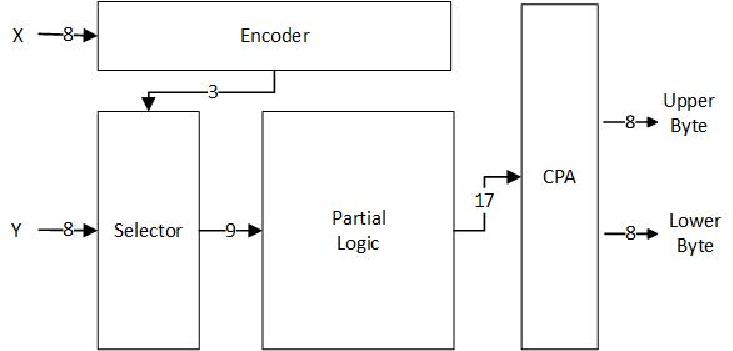
\includegraphics[width=0.4\textwidth]{draw.pdf}
  \centering
  \caption{System Architecture}
  \label{fig:draw}
\end{figure}

Finally, the last part of our design plan is the actual
implementation of the aforementioned modules. 
For the schematic and layout cells to be designed, 
the \texttt{Electric} open-source software \cite{electric} will 
be used. 


\section{Deliverable for the mid-project status report}

Design part :

\begin{itemize}
\item Exploration of the Modified Booth algorithm 
\item Application in the 8-bit multiplier case 
(Truth table, Logic Circuit etc)
\end{itemize}


Implementation part : 

\begin{itemize}
\item Fully designed circuit schematic (\texttt{.ic}, 
\texttt{.sch} cells)
\item Verified correctness of modules (DRC, NCC, ERC)
\item Complete testbenching procedure (ModelSim Simulations) 
\end{itemize}


%\section{Conclusion}
%The conclusion goes here.



% conference papers do not normally have an appendix
% use section* for acknowledgement
%\section*{Acknowledgment}
%The authors would like to thank...


% references section
\begin{thebibliography}{1}

\bibitem{booth}
A. Booth, ``A signed binary multiplication technique'', 
\emph{Quarterly J. Mechanics and Applied}
Mathematics, vol. IV, pt. 2, Jun. 1951, pp. 236-240.

\bibitem{macS}
O.~MacSorley, ``High-Speed arithmetic in binary computers'', 
\emph{Proc. IRE}, vol. 49, pt. 1, Jan. 1961, pp. 67-91.

\bibitem{tb}
Weste and Harris, \emph{CMOS VLSI Design}, $4^{th}$ edition, Addison-Wesley, 2011.	

\bibitem{electric}
Electric open-source EDA system,
\href{http://www.staticfreesoft.com/}{http://www.staticfreesoft.com/}.


\end{thebibliography}

% that's all folks
\end{document}

